\documentclass{article}
\title{Coursera Primeros Pasos}
\usepackage{graphicx}
\usepackage{caption}
\usepackage{subcaption}
\begin{document}
\maketitle

\newpage
\tableofcontents
\listoffigures
\listoftables

\newpage

\section{Introduction}
This is a introduction
\subsection{Resumen Ejecutivo}
\subsection{Marco Teorico}
\subsubsection{Procedimiento}
\paragraph{Esto es un parrafo}
Parrafo 1

\subparagraph{Sub parrafo}
Informacion
\section{Listas}
\begin{enumerate}
    \item preparar ingredientes
    \item  cortar
\end{enumerate}
\begin{itemize}
    \item cebolla
    \item  tomate
    \begin{enumerate}
        \item anidacion de listas
    \end{enumerate}
\end{itemize}

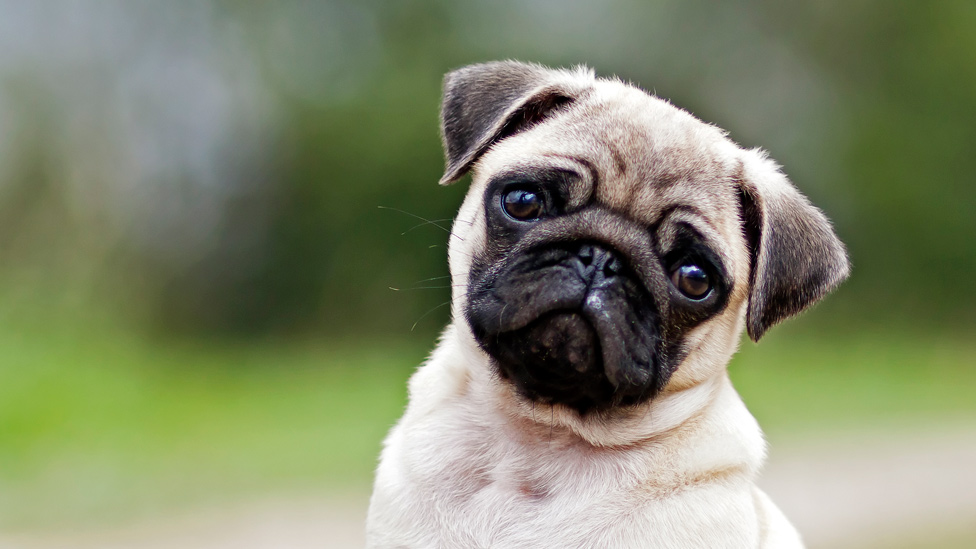
\includegraphics[width = 0.3\textwidth]{Perro.jpg}

\begin{figure}[h!]
    \centering
    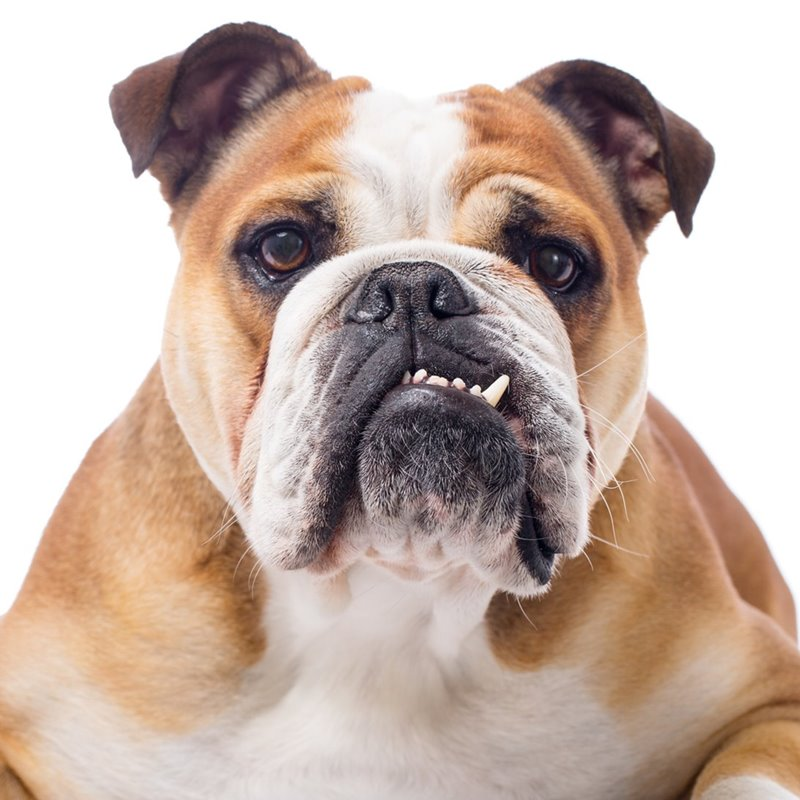
\includegraphics[width = 0.3\textwidth]{Perro2.jpg}
    \caption{Esta imagen es de un perro}
    \label{perro2}
\end{figure}

\begin{figure}
    \begin{subfigure}{0.5\textwidth}
         \centering
         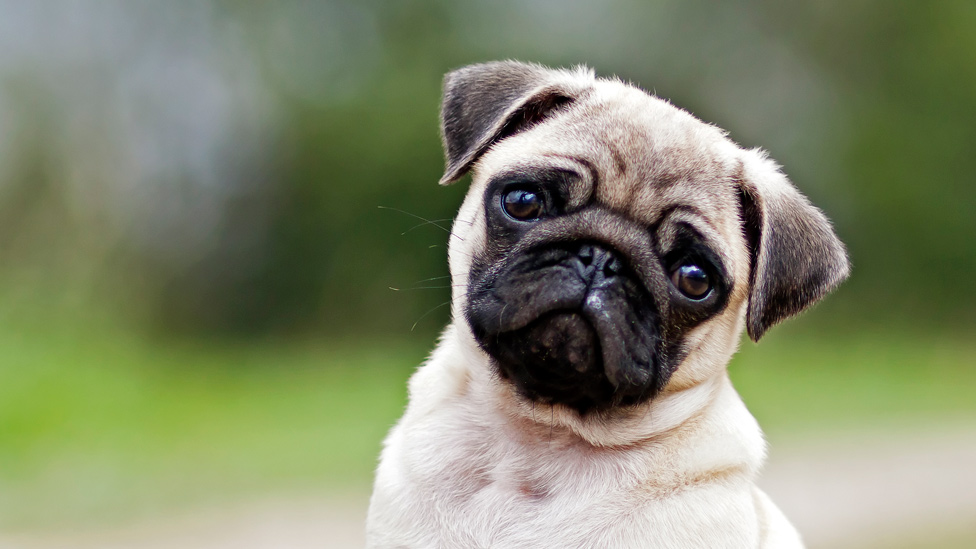
\includegraphics[width = 0.3\textwidth]{Perro.jpg}
         \caption{Imagen 1}
         \label{fig:enter-label}
    \end{subfigure}
    \hfill
    \begin{subfigure}{0.5\textwidth}
         \centering
         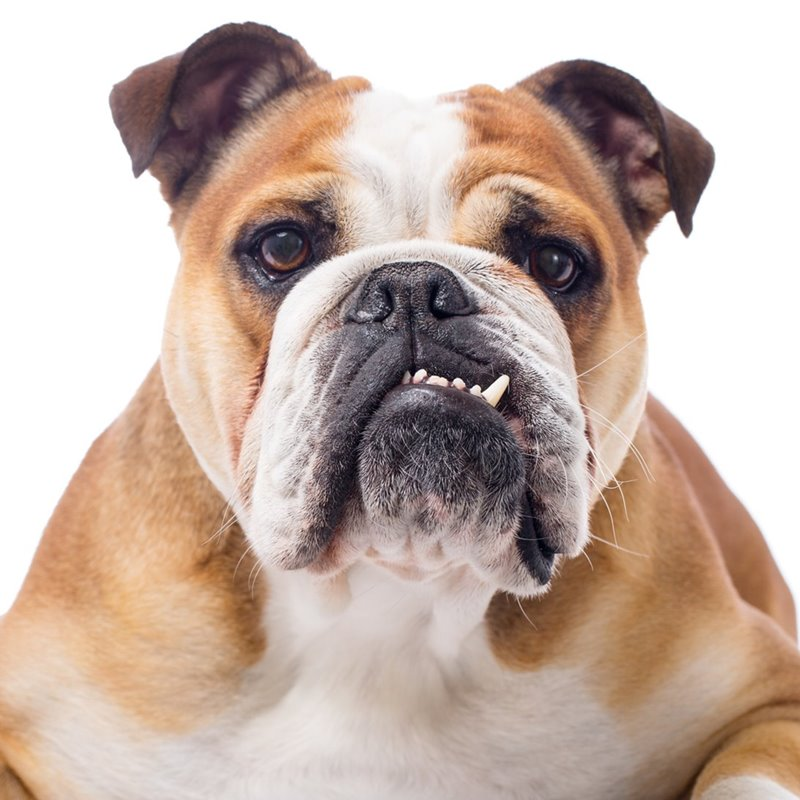
\includegraphics[width = 0.3\textwidth]{Perro2.jpg}
         \caption{Imagen 2}
         \label{fig:enter-label}
    \end{subfigure}
    
    \caption{Imagenes de Perros}
    \label{fig:enter-label}
\end{figure}

\begin{table}[h!]
    \centering
    \begin{tabular}{c|c}
         &  \\
         & 
    \end{tabular}
    \caption{Caption}
    \label{tab:my_label}
\end{table}

\end{document}
